	\documentclass[aspectratio=169]{beamer}

\mode<presentation>
{
\usetheme{Darmstadt}%Darmstadt,Frankfurt

\setbeamercovered{transparent}
}
%Deutsche Silbentrennung
\usepackage[ngerman]{babel}
%Deutsche Umlaute
\usepackage[utf8]{inputenc}
%Listen einr�cken
\usepackage{enumitem}
% font definitions, try \usepackage{ae} instead of the following
% three lines if you don't like this look
\usepackage{mathptmx}
\usepackage[scaled=.90]{helvet}
\usepackage{courier}
%Trennung von deutschen Umlauten
\usepackage[T1]{fontenc}
\usepackage{adjustbox}
\usepackage{url}

\title{Projektarbeit: Háblame - das sprechende Faultier}

%\subtitle{}

% - Use the \inst{?} command only if the authors have different
%   affiliation.
%\author{F.~Author\inst{1} \and S.~Another\inst{2}}
\author{David Artmann\inst{1} \and Dominik Hirsch\inst{1} \and Kristoffer Schneider\inst{1}}

% - Use the \inst command only if there are several affiliations.
\institute[Universities of]
{
\inst{1}
Hochschule für angewandte Wissenschaften\\
Würzburg-Schweinfurt
}

\date{\today}


% This is only inserted into the PDF information catalog. Can be left
% out.
\subject{Talks}



% If you have a file called "university-logo-filename.xxx", where xxx
% is a graphic format that can be processed by latex or pdflatex,
% resp., then you can add a logo as follows:
\pgfdeclareimage[height=0.5cm]{university-logo}{media/logo/fhws.png}
\logo{\pgfuseimage{university-logo}}



% Delete this, if you do not want the table of contents to pop up at
% the beginning of each subsection:
\AtBeginSubsection[]
{
\begin{frame}<beamer>
\frametitle{Gliederung}
\tableofcontents[currentsection,currentsubsection]
\end{frame}
}

% If you wish to uncover everything in a step-wise fashion, uncomment
% the following command:
\beamerdefaultoverlayspecification{<+->}

\begin{document}

% titlepage
\begin{titlepage}
	%Eine mbox wird verwendet um Text zusammenzuhalten
	%vspace erzeugte die in Klammern angegebenen Zeilenabstände
	%baselineskip setzt zeilenabstand
   	\mbox{}\vspace{5\baselineskip}\\
   	%Schriftart und Größe als Attribut
   	\rmfamily\huge
   	%Mittige Textausrichtung (\centerline für eine Zeile)
   	\centering
   	%Das Argument erscheint in Kapitaelchen (small capitals).
	\textsc{Weiterentwicklung von Hablame}
	%Umbruch bezogen auf die Hoehe des Kleinbuchstaben x in diesem Element * Faktor
	\\[3ex]
   	Projektarbeit
   	\rmfamily\Large
   	\vspace{1\baselineskip}\\
   	%Externes einbinden einer Textdatei
   	%% versionsnummer entfernt
   	%\input{version.txt}\mbox{}
	\vspace{3\baselineskip}
	Hochschule für angewandte Wissenschaften Würzburg-Schweinfurt
   	\vspace{5\baselineskip}\\
   	\rmfamily\Large
   	David Artmann\\
   	\rmfamily\Large
   	Dominik Hirsch\\
   	\rmfamily\Large
   	Kristoffer Schneider
   	\vspace{1\baselineskip}\\
   	%Heutiges Datum
   	\today
\end{titlepage}

% toc
\begin{frame}
	\frametitle{Gliederung}
	\tableofcontents
	% You might wish to add the option [pausesections]
\end{frame}

\section{Android}
	\subsection{Motivation und Ziel}
		\begin{frame}
%\frametitle{Gemeinsamkeiten und Unterschiede}
%\framesubtitle{Systemsicherheit}

\begin{block}{}
	example
\end{block}
\begin{block}{}
	more example
\end{block}
\begin{block}{}
	even more example
\end{block}
\end{frame}
		
	\subsection{Aufbau}
			\begin{frame}
\begin{block}{}
	MainActivity.java
\end{block}
\begin{block}{}
	ConversationActivity.java
\end{block}
\begin{block}{}
	RecognitionService.java
\end{block}
\end{frame}
			
	\subsection{Funktionsweise}
			\begin{frame}
	\center{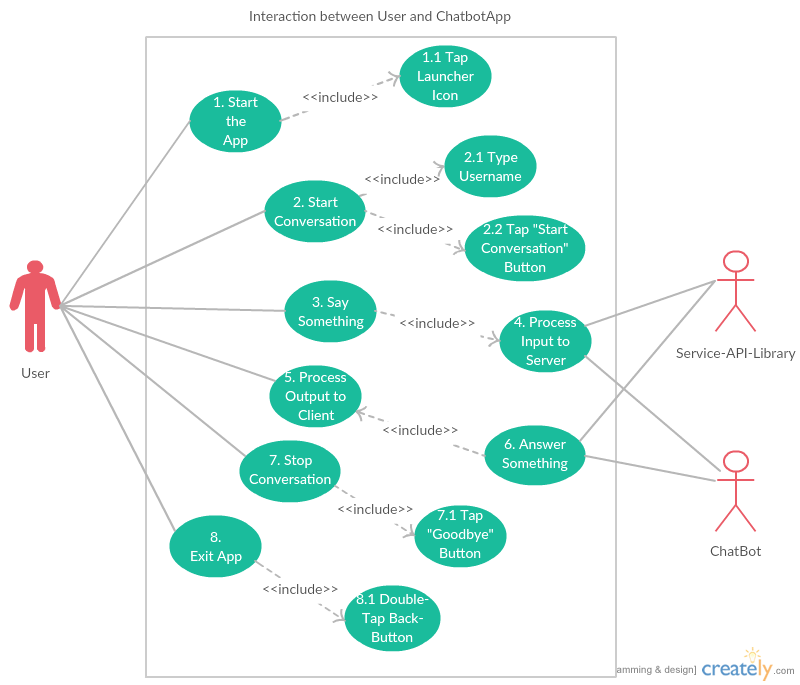
\includegraphics[height=0.5\linewidth]{media/images/android/uc-app.png}}
\end{frame}
			
	\subsection{Design}
			\begin{frame}
%\frametitle{Gemeinsamkeiten und Unterschiede}
%\framesubtitle{Systemsicherheit}

\begin{block}{}
	example
\end{block}
\begin{block}{}
	more example
\end{block}
\begin{block}{}
	even more example
\end{block}
\end{frame}
	
%\begin{frame}
%\frametitle{}

% You can create overlays
%\begin{itemize}
%  \item using the \texttt{pause} command:
%  \begin{itemize}
%    \item First item.
%    \pause
%    \item Second item.
%  \end{itemize}
%  \item using overlay specifications:
%  \begin{itemize}
%    \item<3-> First item.
%    \item<4-> Second item.
%  \end{itemize}
%  \item using the general \texttt{uncover} command:
%  \begin{itemize}
%    \uncover<5->{\item First item.}
%    \uncover<6->{\item Second item.}
%  \end{itemize}
%\end{itemize}
%\end{frame}

\end{document}
